%!TEX root = ../../../adrien_gomar_phd.tex

\subsection{Presentation of the case}

We consider a simplified 
configuration modeling a turbomachinery 
stage. It consists of a 
periodic azimuthal perturbation propagated downstream 
of the inlet boundary of the computational domain. 
The domain is made of two grid blocks in relative 
motion, so that the perturbation, which is steady 
in the upstream block, is seen as unsteady by the 
downstream one.
It is thus representative of 
turbomachinery wakes propagated across an inter-wheel interface.
Figure~\ref{fig:model_tbm_sketch} shows a sketch
of the considered model turbomachinery problem.
\begin{figure}[htp]
  \centering
  \includegraphics*[width=0.25\textwidth]{model_tbm_sketch.pdf}
  \caption{Sketch of the model turbomachinery flow problem.}
  \label{fig:model_tbm_sketch}
\end{figure}

The blocks are generated in cylindrical
coordinates such that the presented configuration
can be assimilated to a slice of 
a turbomachinery stage.
Without loss of generality, 
we set the rotation velocity of the upstream block to zero (stator). 
The stator is composed of $B_{stator} = 10$
"virtual" blades and the rotor of $B_{rotor} = 12$ ones.
The stator's pitch is therefore larger than the rotor's.
These are termed "virtual" blades as no blade is actually meshed.
The pitch ratio is representative of 
contra-rotating open rotor applications in which 
the first row contains more blades 
than the second one. Indeed, in
contra-rotating open rotor applications, the number
of blades is typically smaller than classical
turbomachinery configurations.

A wake is axially injected at the inlet of the
turbomachinery model problem following the \citet{Lakshminarayana1980}
similarity law.



\subsection{Numerical Setup}

The flow is modeled using the 
Euler equations in order to avoid wake thickening and vanishing
associated with viscous effects. 
The velocity is not imposed at the inlet directly
but rather through the total pressure and 
the total enthalpy distributions
\begin{equation}
  \label{eq:rotatingblocks_ptot}
    p_{i0} (\theta) = p_{i_{ref}} \left[1 - 
        \Delta p_i \cdot e^{
          -0.693 \left( 2 \frac{\theta}{L} \right) ^ 2}\right],
\end{equation}
\begin{equation}
  \label{eq:rotatingblocks_htot}
    h_{i0} (\theta) = h_{i_{ref}} \left[1- 
        \Delta h_i \cdot e^{
          -0.693 \left( 2 \frac{\theta}{L} \right) ^ 2}\right],
\end{equation}
where $p_{i_{ref}}$ is the inlet reference total pressure, $\Delta p_i$ the total pressure
deficit in the wake,
$h_{i_{ref}}$ the reference total enthalpy, $\Delta h_i$ the total enthalpy
deficit in the wake and $L$ the wake width.
To impose a realistic distortion, the total pressure and
enthalpy deficits are estimated from a separate turbomachinery simulation.
This leads to $\Delta p_i = 0.025$ and 
$\Delta h_i = - 0.007$.
The negative sign is due to overturning in the wake, which
is due to velocity composition, and therefore specific to rotors.
The static pressure $p_{s_1}$ is imposed at the outlet
\begin{equation}
    p_{s_1} = \frac{p_{i_{ref}}}{\left(1 + 
    \frac{\gamma - 1}{2} M_{0}^2 \right) ^ {\frac{\gamma}{ \gamma - 1}}} ,
\end{equation}
the mean velocity is thus set by imposing the
target mean Mach number value $M_{0}$.
At the azimuthal boundaries, phase-lag conditions~\cite{Erdos1977} 
are used to take into account the space-time periodicity.

The \textit{elsA}~\cite{Cambier2013} CFD code is used.
Roe's scheme~\cite{Roe1981} along with a second-order MUSCL extrapolation 
is used for the spatial discretization of
the convective fluxes and an implicit backward Euler scheme is used
to march the HB equations in pseudo-time.

Each grid block has a radial extent of five grid points, \emph{i.e.} four cells. 
The azimuthal grid density is similar in the stator and in the rotor blocks
to guarantee a consistent capture of the wake on each side of the interface.
To do so, if $\Delta \theta_{cell}$ denotes the azimuthal length of a cell
at the interface, then
\begin{equation}
   \Delta \theta_{cell} = \frac{2\pi}{B_{stator}}~\frac{1}{N_{stator}}
   = \frac{2\pi}{B_{rotor}}~\frac{1}{N_{rotor}},
   \label{eq:az_spatial_discretization_1}
\end{equation}
where $N_{stator}$ and $N_{rotor}$ are the number of cells
in the stator and the rotor, respectively. 
Several wake thicknesses will be tested below
from 30\% down to 1\% of the pitch. For this thinnest wake, 
mesh convergence
is obtained with 500~cells in the azimuthal direction of
the stator, which gives
600~cells for the rotor block.
30~grid points are put in the axial direction. Moreover, a constant
aspect ratio of 5 with respect to the azimuthal length of the cells is
kept, which sets the axial length of the case.
This leads to a total number of grid points of approximately 
170,000. 

Convergence of the iterative procedure used to solve the HB equations is achieved 
after 3,000 iterations for 
all the simulations. 

\subsection{Spectral convergence study}
The primary interest in this section is the wake capturing capabilities of the 
Fourier-based time methods in the rotating part. 
To analyze this, two error measures are defined and
evaluated. 

\paragraph{Spatial-spectrum based error measure}
\label{sec:crit_1}
Initially, we propose an error measure ($\varepsilon_1$) based 
on the loss of signal energy
induced by the HB method at the interface. 
In fact, in the stator part, the wake is steady and is thus not
filtered by the HB operator. 
Conversely, in the rotor part, the wake becomes
unsteady due to the relative speed difference between the
stator and the rotor. However, only a finite number of harmonics~$N$
is used to describe the unsteady field, hence the filtering.

The first error quantification is set up to quantify this filtering 
by using only spatial information and is defined as the $\mathcal{L}_2$-norm 
applied on the 
difference between the rotor and the stator spectra.
It is equivalent to the analytical truncation error 
defined in Eq.~\eqref{eq:def_truncation_error}. 
Indeed, the error is described as the ratio of the unresolved energy 
in the rotor block
to the energy of the full spectrum, 
\emph{e.g.} that of the stator block
\begin{equation}
    \varepsilon_1(N) = \sqrt{
    \frac{\sum_{f=1}^{f_{max}} | \widehat{s}^{~\theta}_N (f) - 
      \widehat{r}^{~\theta}_N (f)|^2}{ 
    \sum_{f=1}^{f_{max}} | \widehat{s}^{~\theta}_N (f)|^2}},
    \label{eq:def_crit_1}
\end{equation} 
where $\widehat{s}^{~\theta}_N$ denotes the spatial Fourier transform (indicated by
the $\widehat{\vphantom{s}.}$ operator) of the azimuthal extraction (shown
by superscript $\theta$) of the result of a HB simulation using $N$~harmonics,
in the stator; $\widehat{r}$ denotes the spectrum of 
the signal transferred to the rotor.
The highest frequency present in the spectrum is dictated 
by the spatial discretization. Thus, $f_{max} = 1 / 2\Delta \theta_{cells}$, 
using the notations of Eq.~\eqref{eq:az_spatial_discretization_1}.
As the azimuthal cell size is similar in both blocks, 
the same sampling is used leading to the same 
frequencies in both stator and rotor spectra.
Details of the algorithm used to compute $\varepsilon_1$ 
are given in Appendix~\ref{app:epsilon_1_steps}.

The azimuthal velocity distributions (left hand-side) and the corresponding spatial
spectra (right hand-side)
are presented in Figure~\ref{fig:spatial_crit} 
for a relative wake thickness of~5\% with respect to the pitch 
and for HB computations using $N=2$, 5, 10 and 18.
\begin{figure}[htp]
  \centering
  \subfigure[$N=2$]{
  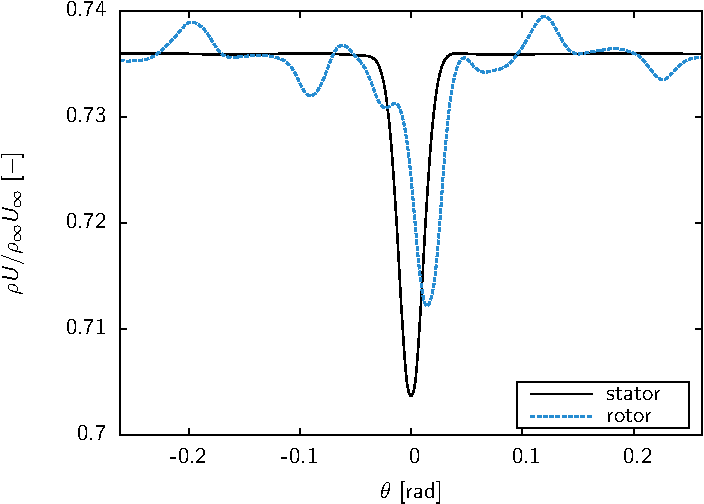
\includegraphics[width=.35\textwidth]{cut_wake_W0490_TSM_N002_adim.pdf}
  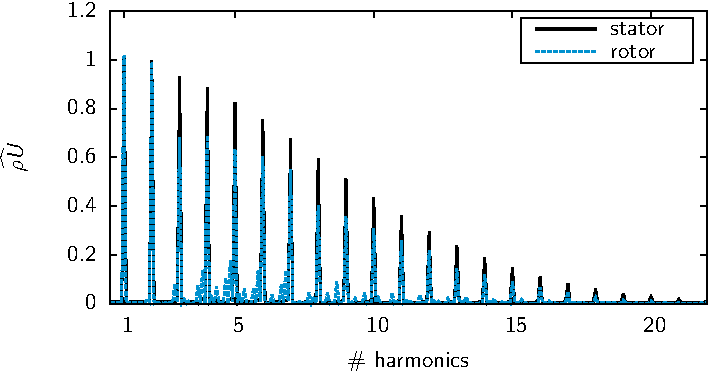
\includegraphics[width=.35\textwidth]{fft_fwake_1D_e490_N02.pdf}}
  \subfigure[$N=5$]{
  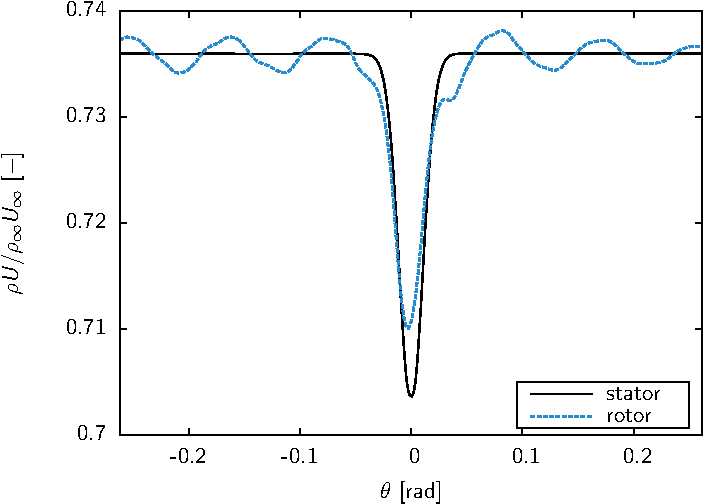
\includegraphics[width=.35\textwidth]{cut_wake_W0490_TSM_N005_adim.pdf}
  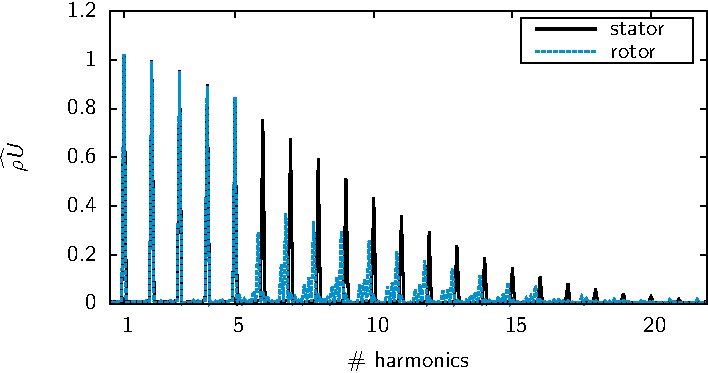
\includegraphics[width=.35\textwidth]{fft_fwake_1D_e490_N05.pdf}}
  \subfigure[$N=10$]{
  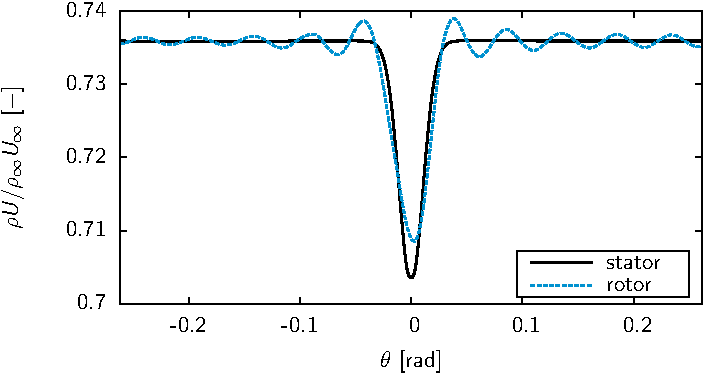
\includegraphics[width=.35\textwidth]{cut_wake_W0490_TSM_N010_adim.pdf}
  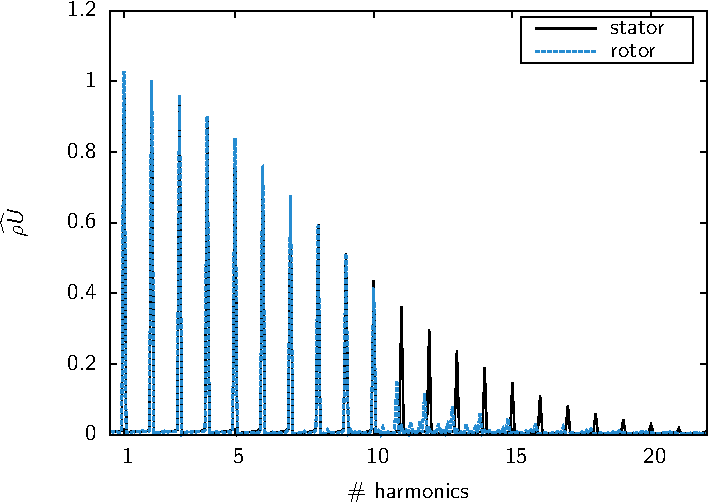
\includegraphics[width=.35\textwidth]{fft_fwake_1D_e490_N10.pdf}}
  \subfigure[$N=20$]{
  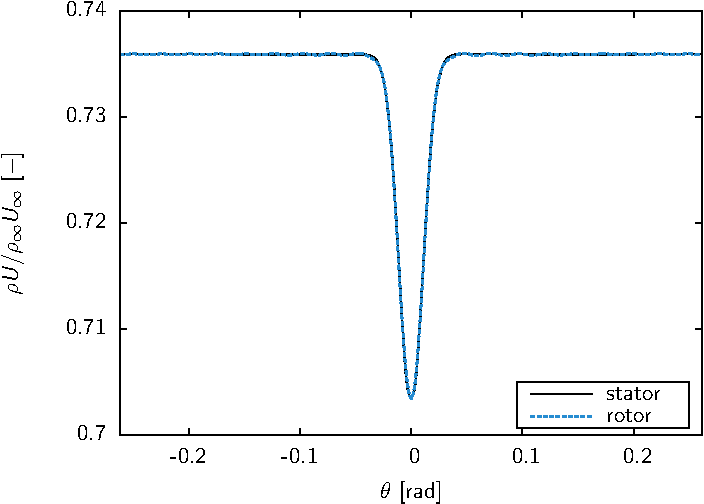
\includegraphics[width=.35\textwidth]{cut_wake_W0490_TSM_N020_adim.pdf}
  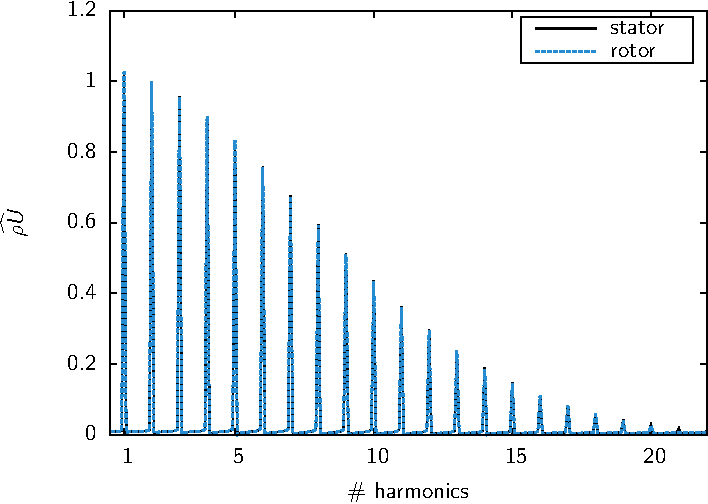
\includegraphics[width=.35\textwidth]{fft_fwake_1D_e490_N20.pdf}}
  \caption{Wake of $L=5\%$ width extracted in stator and rotor 
  blocks. Signal and spatial Fourier analysis for different computations.}
  \label{fig:spatial_crit}
\end{figure}
For the stator, the azimuthal distribution follows a 
Gaussian function as expected. On the contrary, 
the rotor distribution is aliased by the HB discretization 
and exhibits spurious oscillations that tend to disappear
when the number of harmonics used in the computation 
increases.
For $N=10$, some oscillations are still present, 
but the wake captured in the moving block begins to 
converge to that leaving the upstream block.

Inspection of the spectra suggests the same conclusions.
The amplitude of $\widehat{\rho U}$ 
improves when increasing the number of harmonics.
For $N=20$, the spectrum of the rotor 
block matches that of the stator block.
This is consistent with the theoretical analysis, in which more than 
$N=10$ harmonics are needed to capture the wake with less than $20\%$ 
of error for this particular
wake width (see Figure~\ref{fig:analytic_error_paper}).

The filtering introduced by the HB approach 
acts primarily on the time resolution. 
For under-resolved HB computations, a dissipation error is observed.
This dissipation is not spatially uniform and gives rise to
dispersion errors on the spatial spectrum and to spurious
high-frequencies as shown in 
Figure~\ref{fig:spatial_crit} for HB computations $N=2$ to $N=10$.
These effects vanish when the HB computations converge,
\emph{i.e.} for $N \geq 10$.
Therefore, the spectrum of the unresolved spurious frequencies 
is imposed to have a zero amplitude value to compute
$\varepsilon_1$.

In summary, for this wake thickness, the temporal filtering 
on a simulation involving less than ten harmonics is too harsh and leads 
to a significant amount of unresolved energy, 
which deteriorates the numerical representation
of the wake.

For a more quantitative analysis, we compute the error measure
$\varepsilon_1$ for each computation ranging over different 
wake thicknesses and numbers of harmonics. 
Results are summarized in Figure~\ref{fig:crit_1_3d}.
\begin{figure}[htp]
    \centering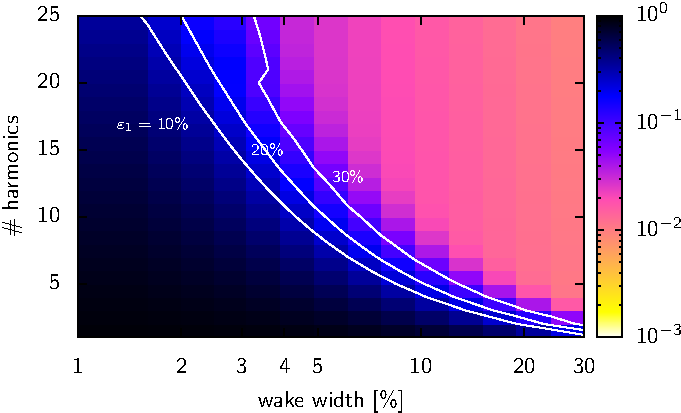
\includegraphics[width=.5\textwidth]{error_crit_1.pdf}
  \caption{Evaluation of the error due to the wake 
  capturing using the first error quantification $\varepsilon_1$.}
  \label{fig:crit_1_3d}
\end{figure}
Because it quantifies the unresolved energy in 
comparison to the resolved energy, $\varepsilon_1$ 
exhibits a behavior similar to that of 
the theoretical error $\varepsilon_{th}$ for a Gaussian function 
(Figure~\ref{fig:analytic_error_paper}).
The iso-error contours have a similar shape 
compared to the analytical ones. 
The conclusions are equivalent: the truncation error decreases with 
the wake thickness and with the number of harmonics used to capture the wake.
Nevertheless, for thicker wakes and higher numbers of harmonics, 
the error measure $\varepsilon_1$ is over-estimated. 
For instance, around $N=15$ and for $L=25\%$,
$\varepsilon_1 \approx 10^{-2}$ whereas the theoretical error $\varepsilon_{th}$
is less than $10^{-4}$. As discussed in the following, the error 
measure $\varepsilon_1$ does not represent a 
realistic measure, because of the spatial 
Fourier transform performed to compute 
the error.

As can be seen in Figure~\ref{fig:ST_discrepancies}, 
the Fourier transform of the spatial signal in the stator block tends to a plateau. 
The thicker the wake, 
the lower the frequency for which the plateau appears: 
approximately 15~harmonics for $L=10\%$
(see Figure~\ref{fig:ST_discrepancies_a}) and 
6~harmonics for $L=25\%$ (see Figure~\ref{fig:ST_discrepancies_b}).
Actually, for a $N$-harmonic HB computation, the spectrum is 
explicitly filtered in the moving block leading to an amplitude 
equal to zero above the $N^{th}$ harmonic. 
Therefore, when the HB computations are converged, the difference between the spatial 
spectra in the stator and in the rotor block is driven by the plateau present 
in the spatial spectrum of the stator block.
\begin{figure}[htp]
  \begin{center}
  \subfigure[$L=10\%$, $N=3$]{
    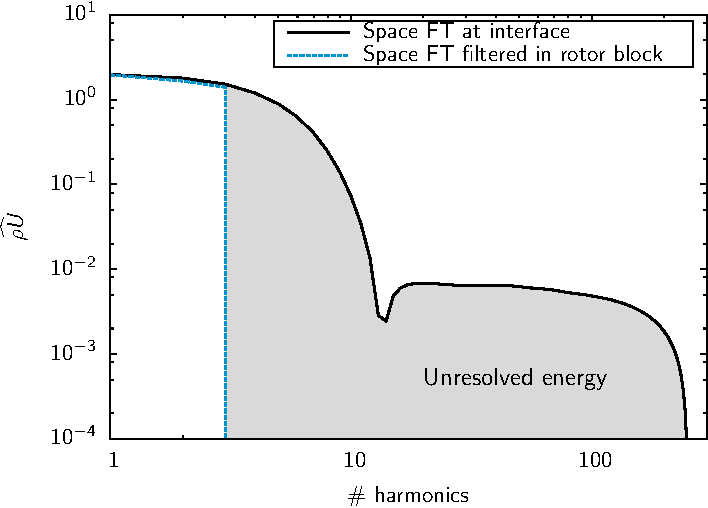
\includegraphics[width=.45\textwidth]{PB_FFT_AZI_10_3}\label{fig:ST_discrepancies_a}}
  \subfigure[$L=25\%$, $N=15$]{
    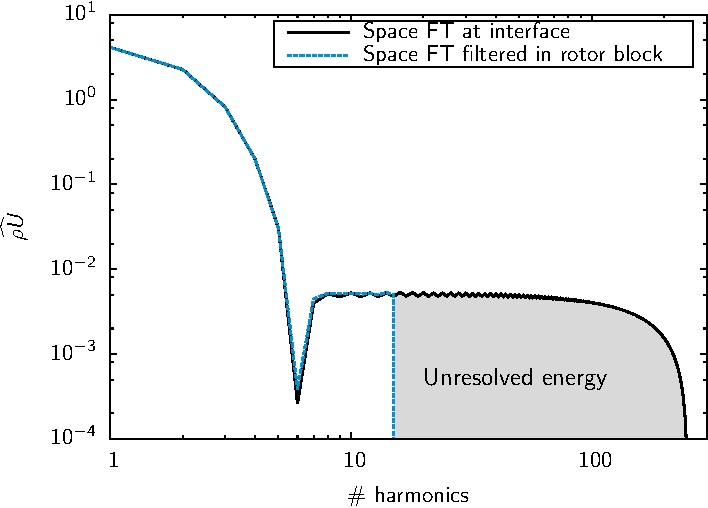
\includegraphics[width=.45\textwidth]{PB_FFT_AZI_25_15}\label{fig:ST_discrepancies_b}}
  \end{center}
  \caption{Discrepancies between spatial and temporal spectra.}
  \label{fig:ST_discrepancies}
\end{figure}

This behavior is linked to the windowing of the signal on 
a bounded interval, namely the pitch. To highlight that, the influence of 
a modification on the inlet boundary condition is analyzed.
The inlet wake distortion used in the model turbomachinery configuration is 
originally based on the analytical Lakshminarayana and Davino 
Gaussian law (see Eq.~\eqref{eq:similarity}). However, 
this law is discretized and imposed on a bounded interval 
that spans the angular pitch. As the relative thickness 
increases, the inlet condition diverges from the analytical 
Gaussian law for which the angular pitch is theoretically 
infinite. This is shown in Figure~\ref{fig:inlet_law_fft} 
through the spectra of three Gaussian laws. The relative 
thickness of the laws are modified through the size 
of the pitch $\Delta \theta$. The multiplication by a factor $100$ 
of the pitch leads to a disappearance of the plateau 
in the spectrum, which accurately matches with the 
Fourier transform of a Gaussian function. 
\begin{figure}[htp]
  \centering
  \subfigure[signal ($\Delta \theta = L$)]{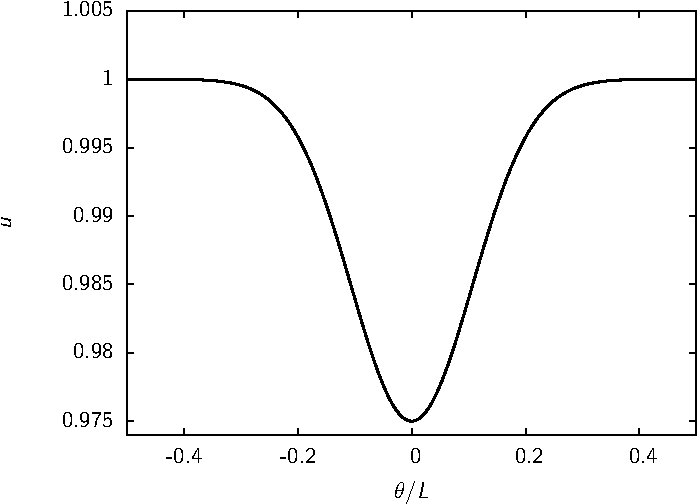
\includegraphics[width=.45\textwidth]{PB_FFT_AZI_DEMO_1_1}}
  \subfigure[Fourier transform ($\Delta \theta = L$)]{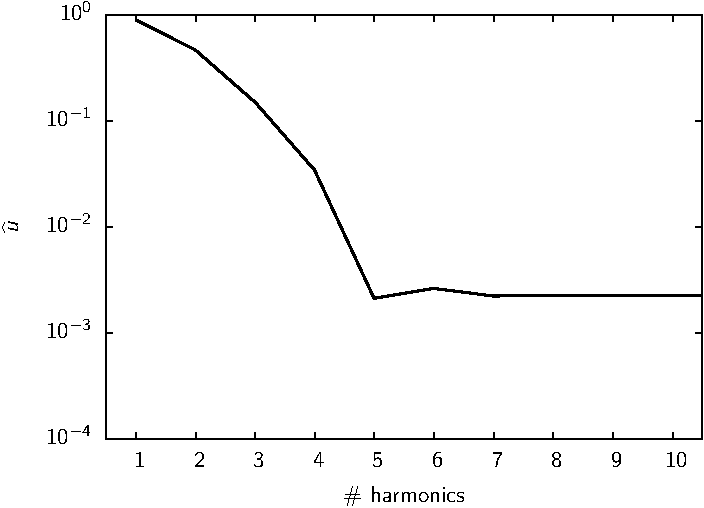
\includegraphics[width=.45\textwidth]{PB_FFT_AZI_DEMO_1_2}}
  \subfigure[signal ($\Delta \theta = 10L$)]{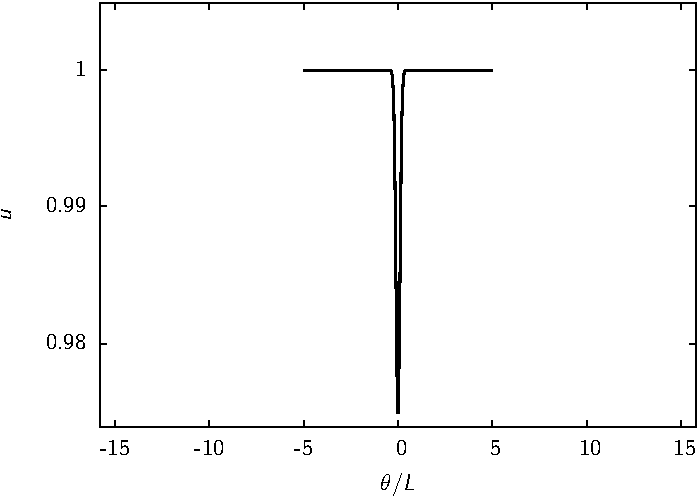
\includegraphics[width=.45\textwidth]{PB_FFT_AZI_DEMO_10_1}}
  \subfigure[Fourier transform ($\Delta \theta = 10L$)]{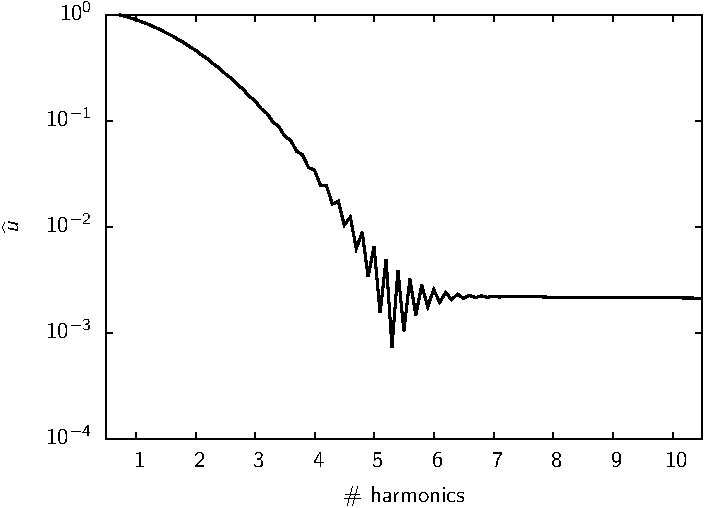
\includegraphics[width=.45\textwidth]{PB_FFT_AZI_DEMO_10_2}}
  \subfigure[signal ($\Delta \theta = 100L$)]{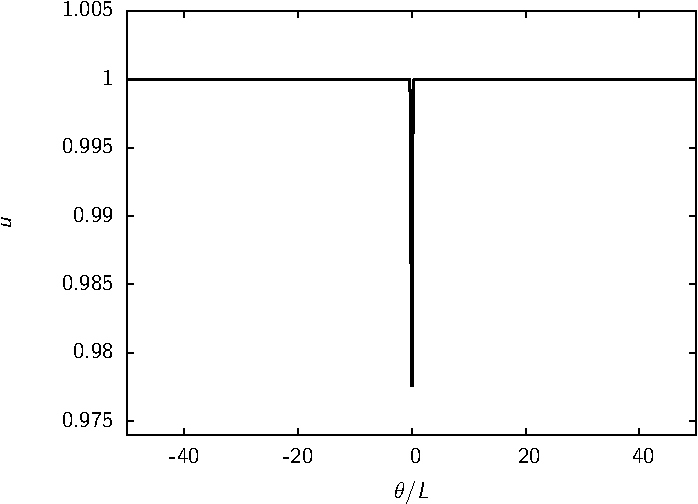
\includegraphics[width=.45\textwidth]{PB_FFT_AZI_DEMO_100_1}}
  \subfigure[Fourier transform ($\Delta \theta = 100L$)]{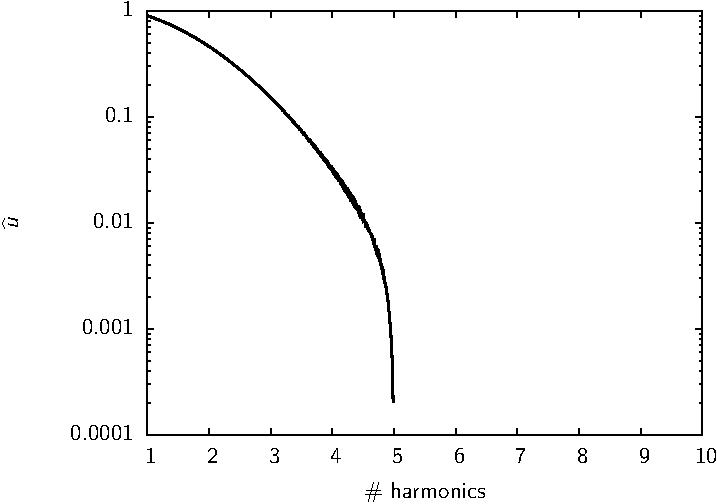
\includegraphics[width=.45\textwidth]{PB_FFT_AZI_DEMO_100_2}}
  \caption{Evolution of the spectrum of the inlet boundary condition for different angular pitches.}
  \label{fig:inlet_law_fft}
\end{figure}

To sum up, a plateau appears in the spatial spectrum of the
stator block. This plateau is explicitly filtered in the
rotor block above the $N^{th}$ harmonic, leading to an over-estimation of the 
first error measure. This over-estimation drives the error value
for higher number of harmonics and thicker wakes.
However, for lower number of harmonics and thinnest wakes, 
the computed error measure is superimposed with 
the analytical one.

\FloatBarrier

\paragraph{Spatial/Time duality error measure}
To get a more realistic error measure, we take 
again into account the energy loss
through the interface, but based on a spatial/time duality. 
As this loss of energy is 
precisely related to the filtering 
introduced on the temporal signal by the HB approach, the second 
error quantification $\varepsilon_2$ addresses the result on 
the temporal information. 

Near the interface of the blocks, consider a fixed observer in
the rotor frame of reference. This observer sees an unsteady 
wake passing as the blocks have a relative speed difference.
The first error quantification has shown the 
influence of the number of harmonics on the spatial signal 
in the rotor block. The spatial/time 
duality error quantification will now
point that this spatial influence is due to a temporal filtering done by
the HB approach.

Following the same notation as in Eq.~\eqref{eq:def_crit_1}, 
the second error measure is written as
\begin{equation}
    \varepsilon_2(N) = \sqrt{
    \frac{\sum_{f=1}^{f_{max}} | \widehat{s}^{~\theta}_N (f) - 
      \widehat{r}^{~t}_N (f)|^2}{ 
    \sum_{f=1}^{f_{max}} | \widehat{s}^{~\theta}_N (f)|^2}},
    \label{eq:def_crit_2}
\end{equation}
where superscript $t$ denotes the temporal version of
the Fourier transform.
By definition, $\varepsilon_2$
quantifies the matching between a spatial signal
and a temporal information.
Again, the error is described as the unresolved energy 
in the rotor block, 
divided by the energy of the full spectrum, 
\emph{e.g.} that of the stator block. 
For $\varepsilon_1$, the amplitude 
of the harmonics above the $N^{th}$ one was imposed to zero. 
On the contrary, for $\varepsilon_2$, the temporal spectrum 
in the rotor block is, 
by essence null above the $N^{th}$ harmonic, as the filtering 
acts on temporal values. 
Details of the algorithm used to compute $\varepsilon_2$ 
are given in Appendix~\ref{app:epsilon_2_steps}.

\begin{figure}[htp]
\centering
  \subfigure[$N=5$]{
  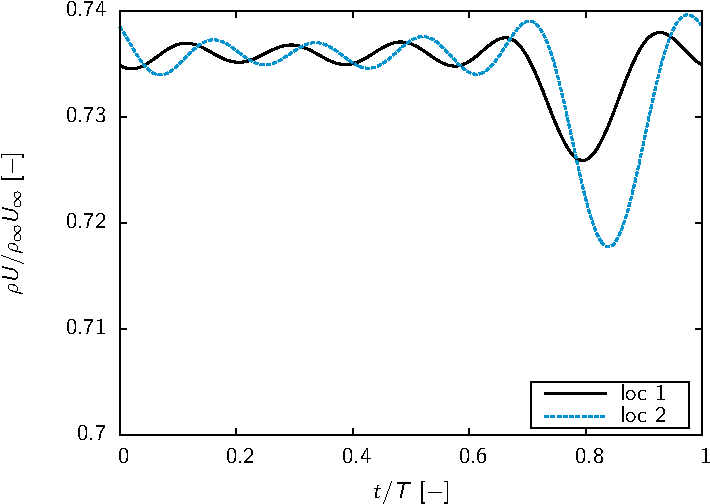
\includegraphics[width=.45\textwidth]{interp_wake_W0490_TSM_N005.pdf}
  \label{fig:temp_signal_a}}
  \subfigure[$N=10$]{
  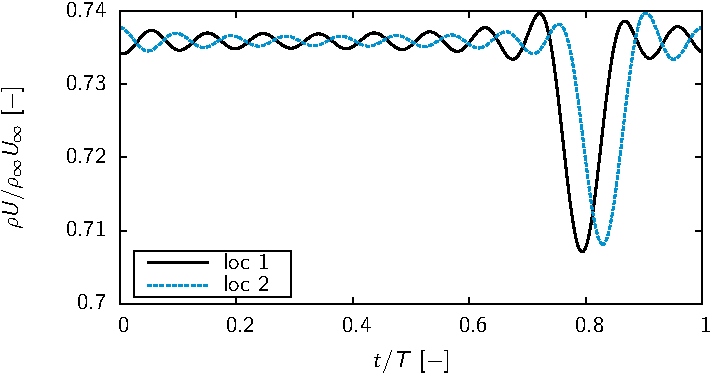
\includegraphics[width=.45\textwidth]{interp_wake_W0490_TSM_N010.pdf}}
  \subfigure[$N=15$]{
  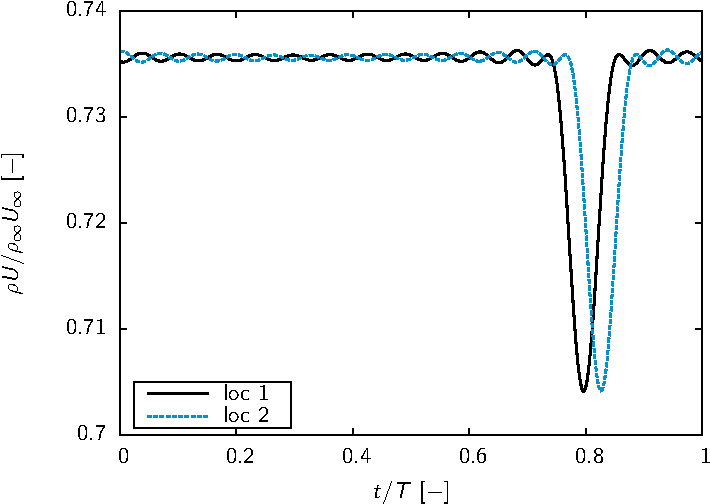
\includegraphics[width=.45\textwidth]{interp_wake_W0490_TSM_N015.pdf}
  \label{fig:temp_signal_c}}
  \caption{Temporal signal seen at loc~1 and loc~2 for a $L=5\%$ wake width.}
  \label{fig:temp_signal}
\end{figure}
Figure~\ref{fig:temp_signal} shows time signals
extracted at two different azimuthal positions at 
the interface of the rotor block, named loc~1 and loc~2. 
The small phase shift between the two 
signals is due to the space lag between the two points, 
and is the same for any choice of the number of 
harmonics used in the computation. On the contrary, 
differences in terms of amplitude are only due 
to the use of an insufficient number of harmonics: 
as the number of modes used for the time 
approximation is increased from $N=5$ to $N=15$, 
the amplitude of the space-shifted signals 
tends to converge to the same value, and 
spurious oscillations tend to disappear. Therefore, in the following,
only loc~1 will be considered.

Figure~\ref{fig:dualite_crit} describes the space and 
time spectra of the axial momentum $\widehat{\rho U}$ at loc~1, 
for computations using $N=2$, 5, $10$ and $20$ 
harmonics and for a wake width of $L=5\%$.
The spatial spectrum contains the whole wavelength 
content associated to the incoming wake; 
on the contrary, due to the filtering introduced 
by the HB approach, the time spectrum is composed of only $N$ harmonics.
\begin{figure}[htp]
\centering
\subfigure[$N=2$]{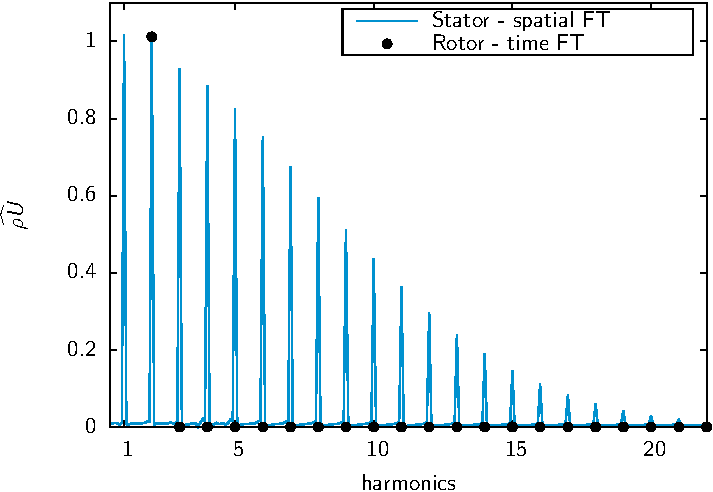
\includegraphics[width=.45\textwidth]{SpcTme_Dualite_0490_02.pdf}}
\subfigure[$N=5$]{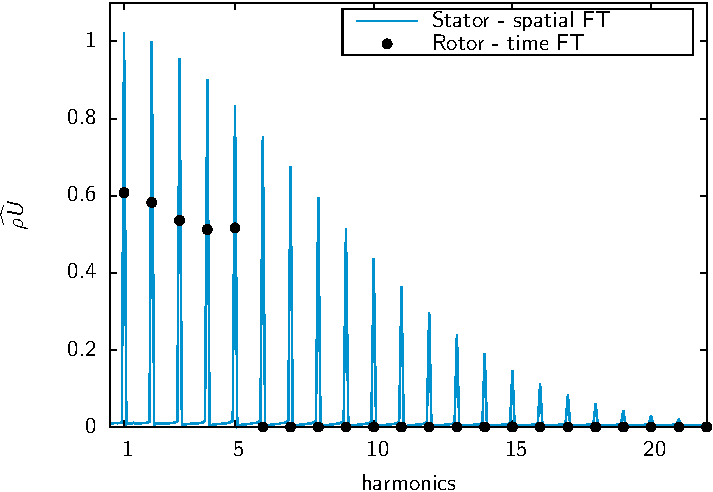
\includegraphics[width=.45\textwidth]{SpcTme_Dualite_0490_05.pdf}}
\subfigure[$N=10$]{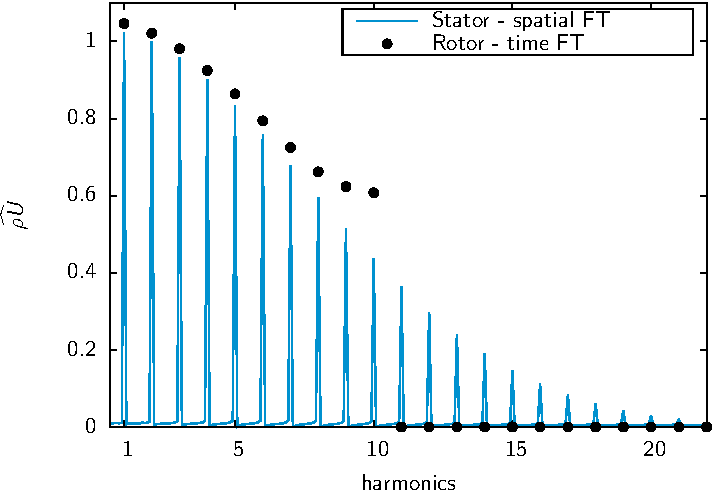
\includegraphics[width=.45\textwidth]{SpcTme_Dualite_0490_10.pdf}}
\subfigure[$N=20$]{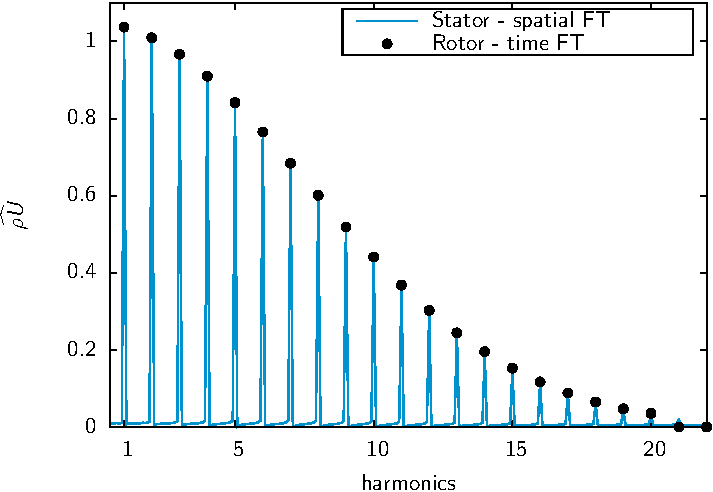
\includegraphics[width=.45\textwidth]{SpcTme_Dualite_0490_20.pdf}}
\caption{Spatial/time duality for a $L=5\%$ wake width.}
\label{fig:dualite_crit}
\end{figure}

For computations using less than 10 time harmonics, 
time spectra are truncated, and the amplitude of 
$\widehat{\rho U}$ differs from that of the corresponding mode in the spatial spectrum.

As the number of time harmonics is increased, 
the amplitude of lower harmonics becomes closer 
and closer to that of the corresponding harmonic 
in the reference signal, and errors move toward 
the higher resolved harmonics. For $N=20$, 
the amplitudes of the 20~resolved harmonics are 
similar for both the time and space spectra.

In summary, the preceding analysis shows that, 
for under-resolved HB computations, the time 
signal is affected by both amplitude and phase errors, 
since the energy content is redistributed incorrectly 
among the resolved harmonics.

To quantify this error, we apply the error measure~\eqref{eq:def_crit_2}
to HB computations of the model turbomachinery 
problem corresponding to different choices 
of the wake thickness and different numbers of 
harmonics. Results are presented in Figure~\ref{fig:crit_2_3d}.
The $\varepsilon_2$ error map is qualitatively 
and quantitatively similar to the $\varepsilon_1$ 
discussed in the previous section. 
Again, the truncation error measured using $\varepsilon_2$ 
for thick wakes and high numbers of harmonics 
does not follow the trend observed with the 
theoretical error $\varepsilon_{th}$, 
due to the spatial filtering introduced at the 
interface by the phase-lag condition.

The preceding analysis shows that, for HB computations 
that are well converged in terms in harmonics, 
the spatial spectrum in the stator and the 
time spectrum in the rotor block tend to match, 
except for additional spatial errors introduced
by the use of an azimuthal Fourier transform on a 
bounded interval, which confirms the 
validity of the error measure defined in Eq.~\eqref{eq:def_crit_2}.
\begin{figure}[htp]
   \centering 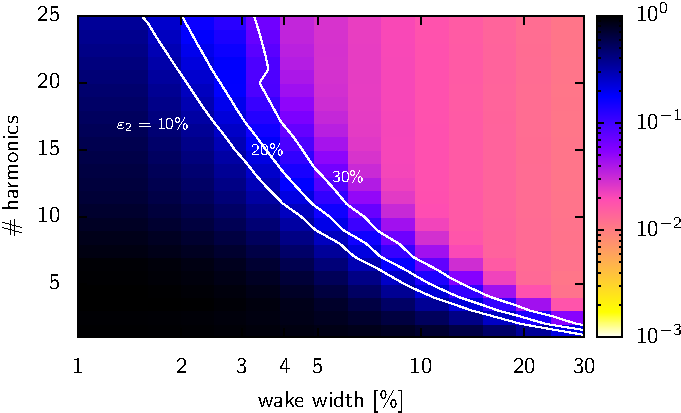
\includegraphics[width=.5\textwidth]{error_crit_2.pdf}
  \caption{Evaluation of the error due to the wake 
  capturing using the second error quantification ($\varepsilon_2$).}
  \label{fig:crit_2_3d}
\end{figure}

\subsection{Comparison with the theoretical error measure}
\label{sub:comp_w_analytic}


The preceding results show that approximated truncation error 
measures computed for the model turbomachinery problem 
using the non-linear Euler equations
exhibit trends, with respect to the wake thickness 
and number of HB harmonics, in close agreement with the 
theoretical error measure derived in Section~\ref{sec:wake_fct}
for a Gaussian function. 
Figure~\ref{fig:error_comp_curves} compares the 
different error measures for HB simulations of 
advected wakes of varying thickness versus 
the number of harmonics used for the time discretization. 
This corresponds to horizontal cuts of Figures~\ref{fig:analytic_error_paper}, 
\ref{fig:crit_1_3d} and~\ref{fig:crit_2_3d}. 
For a wide range of harmonics 
the three error measures are seen to give 
results in very close agreement. For higher harmonics values, 
both the $\varepsilon_1$ and $\varepsilon_2$ error 
measures applied to the model turbomachinery problem 
exhibit a plateau.
The preceding remarks suggest the idea that, 
since all error measure provide similar results, 
at least up to numbers of harmonics of interest for 
practical applicative problems, an \emph{a priori} 
estimate of the number of harmonics required 
to achieve a given error level could be 
obtained by using the theoretical error measure 
Eq.~\eqref{eq:analytical_conv}, if a quick 
estimate of the wake thickness characteristic 
of a given turbomachinery problem is available. 
In the next Section, we show that a reasonable and more general 
estimate can be obtained from a preliminary steady 
computation based on the mixing plane interface condition.
\begin{figure}[htp]
  \centering
  \subfigure[$L = 2 \%$]{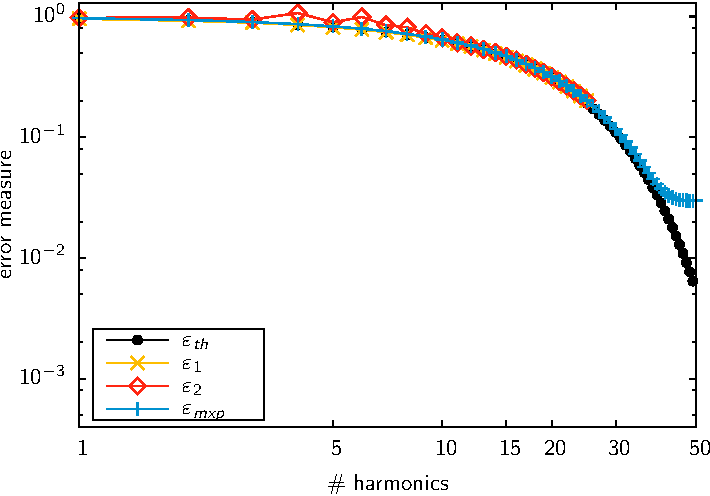
\includegraphics[width=.45\textwidth]{RB_MP_0200_error_logY.pdf}}\quad
  \subfigure[$L = 5 \%$]{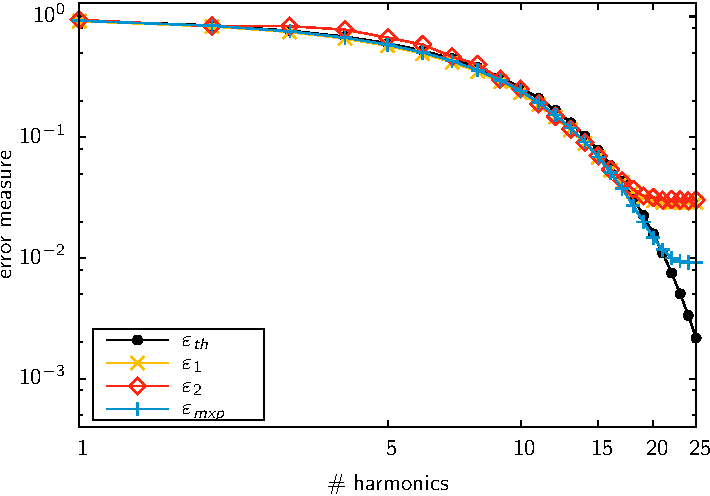
\includegraphics[width=.45\textwidth]{RB_MP_0490_error_logY.pdf}}\quad
  \subfigure[$L = 10 \%$]{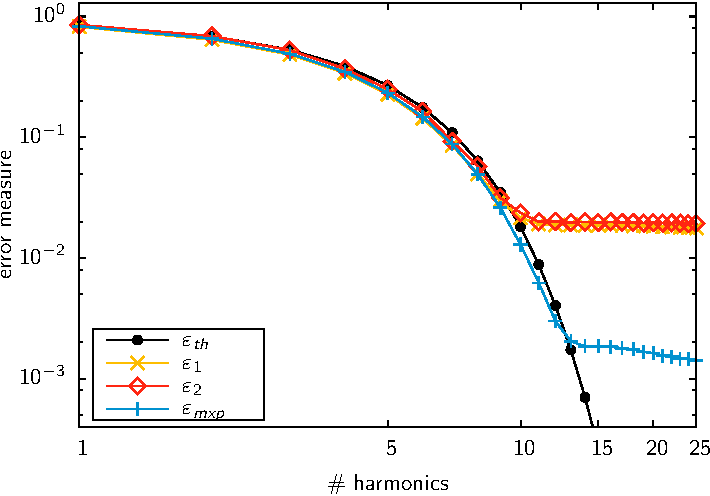
\includegraphics[width=.45\textwidth]{RB_MP_0965_error_logY.pdf}}\quad
  \subfigure[$L = 15 \%$]{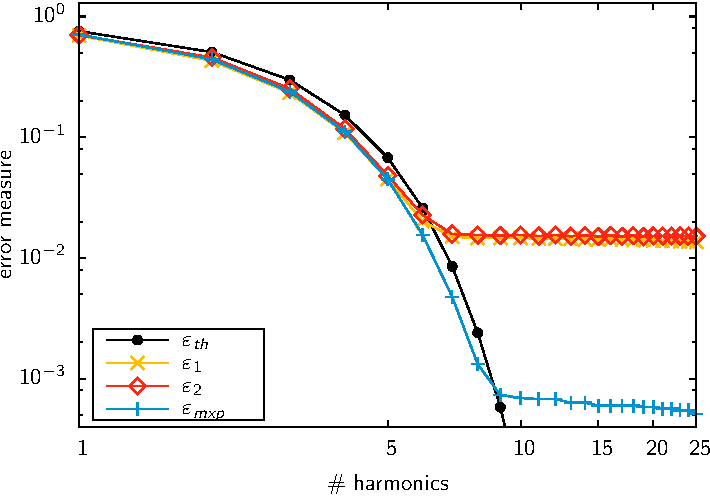
\includegraphics[width=.45\textwidth]{RB_MP_1520_error_logY.pdf}}\quad
  \caption{Truncation, computed and analytical errors for four wake widths.}
  \label{fig:error_comp_curves}
\end{figure}

\subsection{Toward an \emph{a priori} error estimate}
\label{sub:prediction_tool_azimuthal_fft}

In order to define an \emph{a priori} error measure 
that can be used to estimate the number of 
harmonics required to achieve a reasonable 
convergence of the HB method, we suggest to 
evaluate the wake thickness by using a preliminary 
mixing plane steady computation. Indeed, if 
potential effects due to the downstream row can 
be neglected, the spatial information at the interface 
in the stator block, essentially due to the incoming 
wakes, can be captured without taking into account 
the relative motion between the wheels, \emph{i.e.} 
by means of a mixing plane computation. 
Given the approximated azimuthal distribution at 
the stator interface, we consider the cumulative
energy content of the signal up to a given frequency $f$ 
(or, equivalently, to a given harmonic $N=f/f_1$ where $f_1$ is the
base frequency value of the considered unsteadiness,
here the opposite blade passing frequency). 
The cumulative energy is defined as
\begin{equation}
    E(f) = \frac{
      \int_0^f | \widehat{g}(\zeta)|^2 \diff \zeta
    }{
      \int_0^\infty | \widehat{g}(\zeta)|^2 \diff \zeta
    },
\end{equation}
where $\widehat{g}$ is the spectrum of the quantity of interest.
By comparison with Eq.~\eqref{eq:def_truncation_error},
the relation between the relative accumulated energy $E$
and the truncation error $\varepsilon_{mxp}$ is given by
\begin{equation}
    E(f) = 1 - \varepsilon_{mxp}^2 (f).
    \label{eq:correspond_E_error}
\end{equation}


Note that this last error measure is based only on 
the amount of unresolved energy that is left 
in a computation if the spatial signal is 
truncated at a given cutoff frequency $f$, 
and does not require any information from the rotor
block, but it depends only on the characteristics 
of the incoming wake.

To check if the new error measure represents an 
accurate estimate of the truncation error of 
an HB simulation, we carry out again a 
parametric study of the error versus different 
wake thicknesses and numbers of harmonics 
(equivalently, cutoff frequencies), and compare 
the results to those of the \emph{a posteriori} error measures 
obtained for the model turbomachinery problem and for the 
theoretical error $\varepsilon_{th}$. 
Results corresponding to $\varepsilon_{mxp}$ are 
superposed to the corresponding curves in Figure~\ref{fig:error_comp_curves}. 
The \emph{a priori} error measure ($\varepsilon_{mxp}$) matches 
the theoretical estimate ($\varepsilon_{th}$)
and the \emph{a posteriori} measures ($\varepsilon_1$, $\varepsilon_2$)
over a wide range of harmonics. Similarly to the \emph{a posteriori}
errors $\varepsilon_1$ and $\varepsilon_2$, the \emph{a priori} error
exhibits a plateau for high $N$ and high wake thicknesses, 
due to the application of the Fourier transform on a bounded interval. 
We also stress the close agreement between 
$\varepsilon_{mxp}$ and $\varepsilon_{th}$: specifically, 
estimates of the number of harmonics needed to capture 99\% 
of the cumulative energy (equivalently, to get a 
truncation error equal to 10\%) are identical for 
all error measures.

This is indeed very attractive as a preliminary
steady mixing plane simulation is cheaper than
a harmonic balance computation. This tool
will be assessed on two CROR configurations in 
Chapter~\ref{cha:dream_ls_isolated} and applied
in Chapter~\ref{cha:dream_hs_isolated}.
